\documentclass[a4j,11pt]{article}

%
% PDFファイルの作成方法
%
% ・dvipdfmを使う場合
%   dvipdfm -p A4 sample.dvi
%
% ・Adobe Acrobat (Distiller) を使う場合
%   dvipsk -D 600 -t a4 -P pdf sample.dvi
%   psファイルをDistillerでpdfへ変換
%

% ***************
%      注意!
% ***************
% 以下のtxfontsパッケージを使用するとcmフォントが(数式も含めて)Times,
% Helveticaなどに置き換えられます。詳しくは下記のウェブページなどをご参照くださ
% い。
% http://oku.edu.mie-u.ac.jp/~okumura/texwiki/?TXFonts
%
% これを使いたくない方は以下の\usepackage{txfonts}を無効にしてください。
% その場合にはcmフォントがPDFに埋め込まれるのでファイルサイズが多少大きくなります。
\usepackage{txfonts}
\usepackage{url}
\usepackage[notes,backend=biber]{biblatex-chicago}
\usepackage{listings}
\bibliography{references}
% \usepackage{xeCJK}
% \usepackage{CJKutf8}
\usepackage{graphicx}
\graphicspath{{images/}}

% 
% マージン設定(できるだけ変更しないでください)
%
\setlength{\oddsidemargin}{0truemm}
\setlength{\hoffset}{-0.4truemm}
\setlength{\voffset}{-0.4truemm}
\setlength{\textheight}{247truemm}
\setlength{\textwidth}{160truemm}
\setlength{\headheight}{0truemm}
\setlength{\topmargin}{0truemm}
\setlength{\headsep}{0truemm}

\pagestyle{empty}

\begin{document}
\renewcommand{\baselinestretch}{1.12}\small\normalsize

\begin{center}
%   \textbf{\Large 応用物理学会学術講演会予稿のタイトル}
  
  \textbf{\large Leveraging Segmentation of Physical Units through a Newly Open Source Corpus}
  
  \textbf{Luca Foppiano, Akira Suzuki, Thaer M. Dieb, Masashi Ishii and Mikiko Tanifuji}
  
  \textbf{National Institute for Materials Science (NIMS)}
%   \textbf{Research and Services Division of Materials Data and Integrated System (MaDIS), National Institute for Materials Science (NIMS), 1-1 Namiki, Tsukuba, Ibaraki 305-0044, Japan}
  
  \textbf{E-mail: ISHII.Masashi@nims.go.jp}
\end{center}

%0.2\cdot e\textsuperscript{3}$

%The ability to correctly parse and normalise physical measurements is a task common in almost every domain. 
The identification of physical measurements is a recurrent need in material informatics (MI). For example, the extraction of superconductor materials and their properties requires to identify and understand temperature, pressure, magnetisation \autocite{foppiano2019proposal}.
When designing automatic systems for information extraction from scientific literature, the identification of the raw measurement alone is not sufficient. Parsing and understanding of units and values are required for transformation (such as normalisation). 
%In polymers, the standard unit does not correspond with the one in the Polynfo reference database (e.g. \textit{specific volume} is standardised as  \( \frac{m\textsuperscript{3}}{kg} \) but is represented in Polynfo with \( \frac{cm\textsuperscript{3}}{kg} \).
However, quantities and units are contained in unstructured text with ad-hoc conventions to convey their meaning: it is common to encounter new variations or more complex units which are not present in any general dictionaries. String matching and lookup are not working with the growing unit complexity. A generic unit segmentation system is, therefore, necessary.

This contribution is part of a larger project called Grobid-quantities \autocite{grobid-quantities}, a machine learning (ML) based, Open Source system for extracting and normalising physical measurements from scientific and patent literature. 
%Grobid-quantities is a module based on Grobid \autocite{GROBID}, a machine learning framework for parsing and structuring PDF documents. 
In this submission, we present a general approach for units representation, and we introduce the public availability of a corpus of segmented physical units. 
%Corpora of this kind are needed for training newly sequence labelling unit segmentation models or to evaluate existing systems. 
% There are several work related on extraction of physical units. \textit{Berrahou et all}\autocite{berrahou2013extract} illustrates a fairly similar model for unit representation without taking in account the needs of unit normalisation. \textit{Peter et all}\autocite{peter2017quantity} describes the construction of a database of units using machine learning. Unfortunately they do not provide the resulting database publicly. 
Currently, there are no comparable results in scientific literature because no public dataset is available for this task.
Our approach for unit representation follows the International System of Measurement (SI), where each complex unit is represented as a product of triples: \textit{prefix}, \textit{base} and \textit{power}. We use XML to identify the various blocks of the triples in the original text in a way to have enough information to populate the unit according to the model.
%For example \texttt{kV/cm\textsuperscript{2}}, corresponds to \texttt{$kV\cdot cm\textsuperscript{-2}$} and becomes \texttt{[(k, V, 1), (c, m, -2)]} as product of triples. 
%The corpus is distributed in XML  labels corresponding to the three element of the triple. 
%The XML representation is the intermediate step between natural language and model representation. 
%The example previously illustrated is then encoded in XML as \texttt{\small{<unit><prefix>k</prefix><base>V</base> <pow>\char`/</pow><prefix>c</prefix><base>m</base><pow>2<pow></unit>}}.  
Figure~\ref{fig:dataset example} illustrate an example on how \texttt{kV\textsuperscript{2}/cm} is represented in XML and in the abstract model. 
\begin{figure}[h]
    \centering
    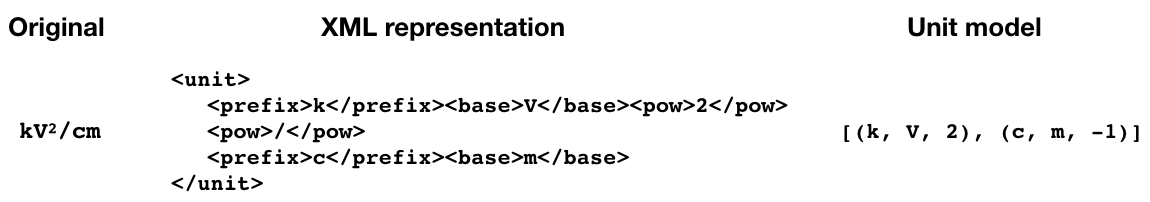
\includegraphics[width=0.9\textwidth,natwidth=575,natheight=101]{sample-corpus.png}
    \caption[Example of the dataset] {Example of unit representation in the original text, XML and abstract model. Notice that \texttt{<pow>} is used to identify both exponent and division marks (needed to correctly set the second triple exponent, in this case negative).}
    \label{fig:dataset example}
\end{figure}

The corpus was created using data extracted in previous work by some of the authors \autocite{suzuki2018constructing}, where about 2000 units were extracted from 3490 papers of Journal of Applied Physics. The data was pre-annotated using an existing ML model for Unit segmentation in Grobid-quantities, and manually corrected. This dataset contains approximately 700 simple and 1300 complex units, it's available at the Grobid-quantities documentation\footnote{\url{https://grobid-quantities.readthedocs.io/en/latest/references.html}}, together with the description of the XML schema\footnote{\url{https://grobid-quantities.readthedocs.io/en/latest/guidelines.html#units-crf-model}}.

We provide, with this contribution, an Open Source corpus to leverage the development of unit segmentation systems. It provides enough data to train new models, or for evaluation of any ML or Rule-based systems, using a standard and comparable ground. 

\end{document}